\chapter{Discussion}\label{chap:discussion}

In this chapter, we discuss the findings of this thesis presented in Chapter
\ref{chap:results}, which we will summarize in Section \ref{sec:key_findings}.
We then formulate a set of recommendations in Section
\ref{sec:discussion_recommendations}, and finally highlight some limitations and
future directions of research in Section \ref{sec:discussion_limitations}.

\section{Key Findings}\label{sec:key_findings}

Overall, we found that \acrshort{mmd}s show high correlation coefficients on
graphs extracted from proteins (see Section \ref{sec:overall_behaviour}). This
finding is somewhat surprising considering recent findings indicating that
\acrshort{mmd} seems often me unstable on synthetic graphs such as Erd\"os-Rényi
graphs, Watts-Strogatz graphs, and Barabási–Albert graphs under some
combinations of perturbation types, kernels and descriptors
\citep{obray2022evaluation}. While we found configurations of MMD with
low correlations and high $\sigma_\MMD$ (see for instance Figure
\ref{fig:mmd_consistent_eps} upper left pane with the degree histogram and the
Weisfeiler-Lehman kernel-based MMDs where protein graphs are subject to
rewiring, see Figure \ref{fig:wlk}), such \acrshort{mmd} configurations were not
prevalent. We hypothesize that this is due to the highly structured nature of
the graphs used in this thesis (see Figure \ref{fig:er_comparison_8a_graph} for
an example).

\begin{figure}
  \centering
  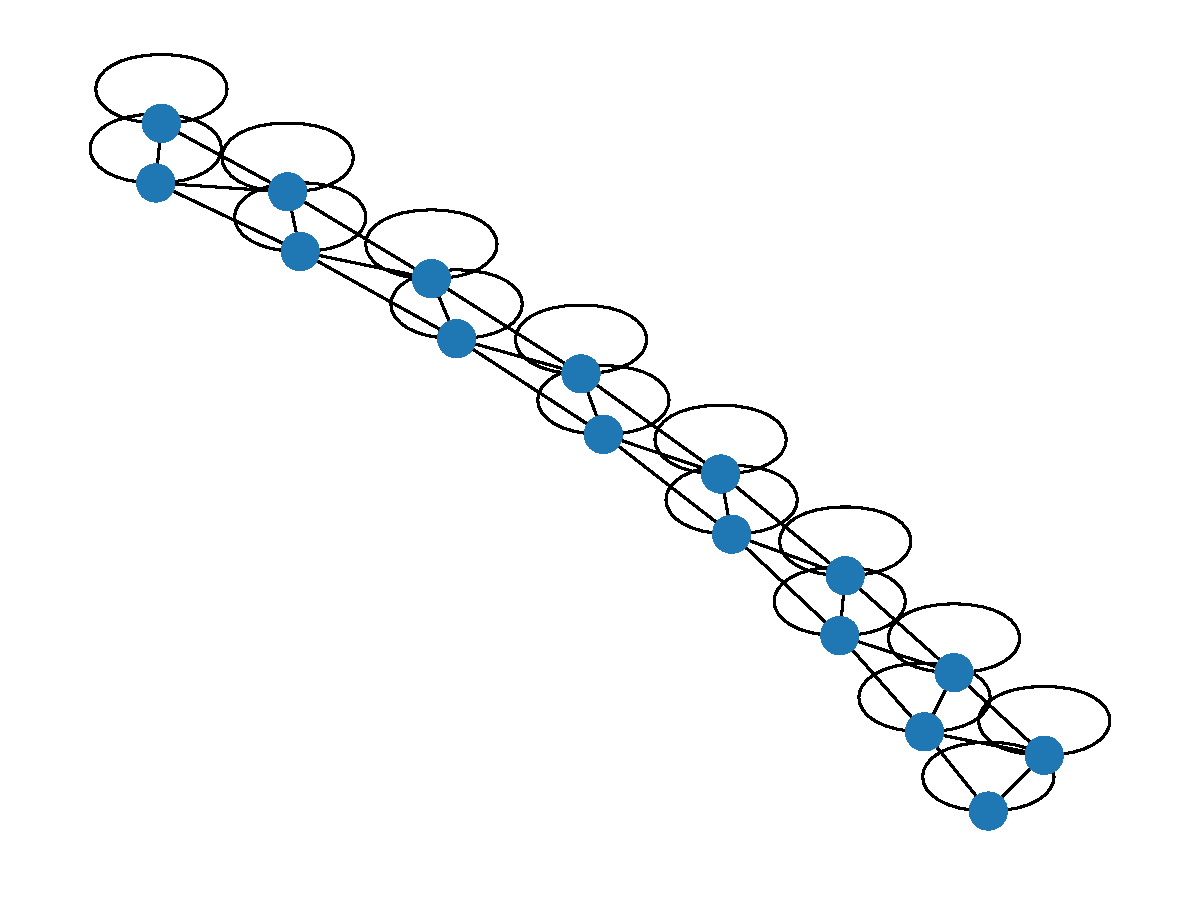
\includegraphics[width=0.4\textwidth]{./figures/results/8_a_graph.pdf}
  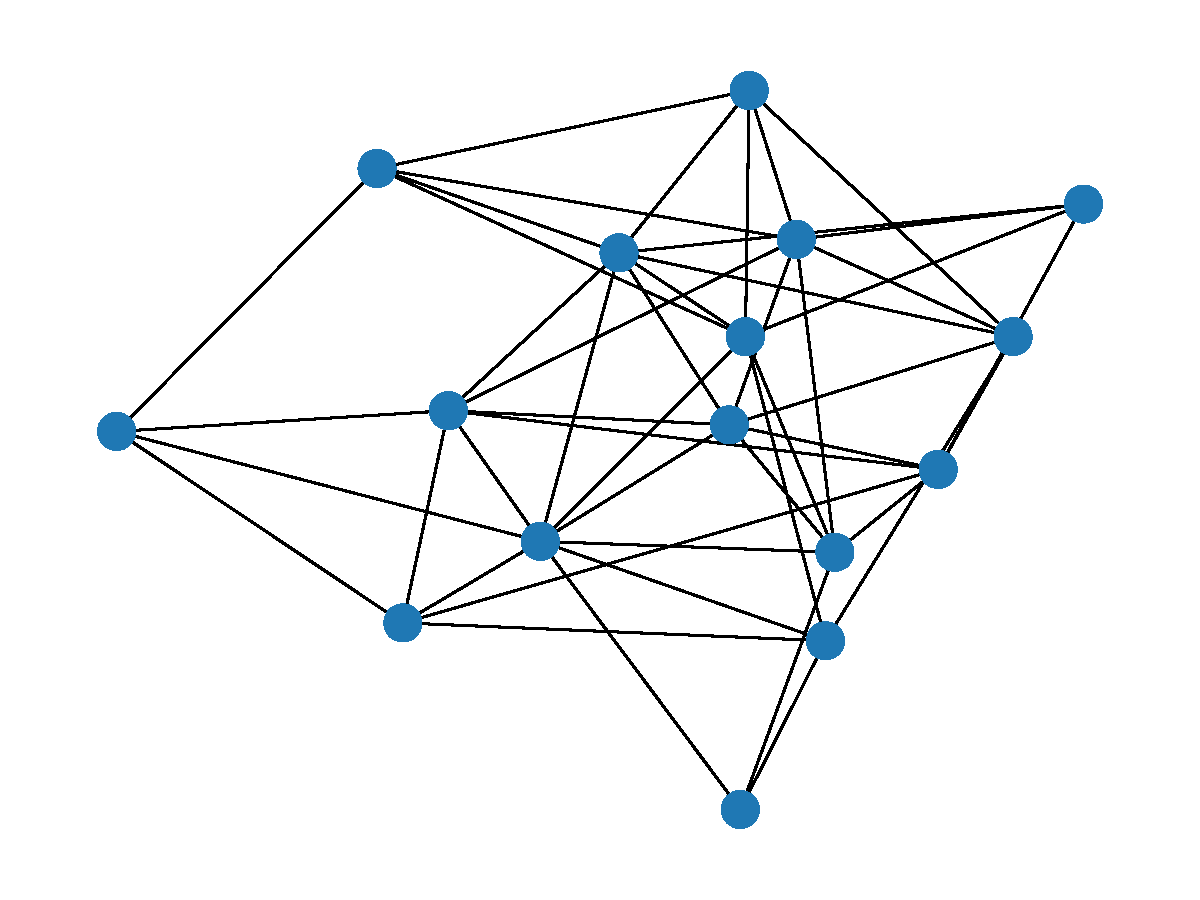
\includegraphics[width=0.4\textwidth]{./figures/results/er_graph_8_a_params.pdf}
  \caption[Example 8-\si{\angstrom}-graph vs Erd\"os-Rényi graph with the same
number of nodes and edges.]{Example 8-\si{\angstrom}-graph extracted from a
protein versus Erd\"os-Rényi graph with the same number of nodes and edges. The
protein entry used here to obtain the 8-\si{\angstrom} graph is an
uncharacterized protein (UniProtKB ID: A0A6Q8PFQ6). We chose this protein for
illustrative purposes because it was the shortest protein found in the human
proteome as predicted by the AlphaFold2 model. The self-loops shown in the
protein graph are present in all graph extraction techniques used in this
thesis.}
  \label{fig:er_comparison_8a_graph}
\end{figure}

Furthermore, we found that the correlation coefficients and standard deviation
of \acrshort{mmd} configurations were greatly influenced by the graph
representation extracted from the protein. Namely, for $\varepsilon$ graphs
(which overall seemed more stable than $k$-NN graphs, see Figure
\ref{fig:correlations_graph_construction}), the higher the $\varepsilon$ value
to extract the graph, the lower the correlation to the perturbation applied
(Figure \ref{fig:mmd_sensitivity_eps}).

Next, we introduced in Section \ref{sec:descriptors} two \emph{novel}
protein-specific descriptors that can be used in \acrshort{mmd}. In Section
\ref{sec:results_protein_descriptors}, we show that those descriptors are both
fast to compute (Table \ref{tab:runtimes}) and are able to detect point cloud
perturbations with high fidelity (Figure \ref{fig:protein_specific_descriptors},
see also Section \ref{sec:results_protein_descriptors} for a more detailed
discussion).


We found that the Weisfeiler-Lehman kernel, introduced in Section
\ref{sec:methods_kernels} applied to \acrshort{mmd} was able to detect
perturbations unable to be detected by traditional graph descriptors such as
point mutations, which are relevant for the protein domain (see Section
\ref{sec:results_graph_kernels}). However, the resulting MMD meta metrics
obtained using the Weisfeiler-Lehman kernel were not as high as for other MMD
configurations used in this thesis (see Section \ref{sec:quality_wl} for a
detailed examination). Furthermore, we found that Weisfeiler-Lehman-based MMD
configurations are not sensitive (i.e. the normalize MMD does not increase) when
lower levels of perturbation are applied (see Figure \ref{fig:wlk}). This can be
alleviated by using an alternative descriptor such as the ESM protein embedding
introduced in Section \ref{sec:evalproblem}, which is more sensitive (i.e.
requires less perturbation to reach higher normalized MMD values) to lower rates
of point mutation (see Figure \ref{fig:esm_descriptor}).

We analyzed the \acrshort{mmd} obtained from kernels operating on persistence diagrams in
Section \ref{sec:results_topo_kernels}, which show excellent meta metric performance since
\acrshort{mmd} values leveraging topological kernels both exhibit high correlations to
point cloud perturbations and low $\sigma_\MMD$. While unable to detect
point mutations, we propose an alternative to be topological investigation of such point
clouds in Section \ref{sec:tda_limitations}.

\section{MMD in Practice: Recommendations}\label{sec:discussion_recommendations}

Leveraging those key findings, we now formulate a set of recommendations for a
practitioner who needs to evaluate a generative protein model using one of the
protein representations highlighted above.


\subsection{Setting Up Appropriate Baselines}\label{sec:discussion_baselines}

Overall, we advise the practitioner to carefully evaluate certain baselines when
possible. The first baseline would be to evaluate the \acrshort{mmd} between
different i.i.d. samples of the reference distribution to establish the range of
\acrshort{mmd} to be expected in the best case, which we refer to as the
\emph{positive control}. We conducted such positive controls for various MMD
configurations in Appendix \ref{sec:mmd_baselines}. From there, an accurate
assessment of the quality of the model can be made. If the kernel and data
representation allows it, it is also advisable to establish a \emph{negative
control}. This would show the worst possible performance between any two
distributions. If this is not possible, as is the case in this thesis (e.g.
there is no negative control for all \acrshort{mmd} values perturbed using the
Gaussian noise), it is useful to examine cases of extreme perturbations and
compare the resulting \acrshort{mmd} values to those. Such an assessment can
provide a surrogate for the negative control and confers a sense of scale for
the particular problem tackled. As with discriminative models, it is also useful
to compare the MMD obtained from the generated model with other MMDs obtained
from other models used in the literature to make comparative benchmarks of
performance. In such a context, taking into account the values of $\sigma_\MMD$
to establish the robustness of a particular MMD configuration is important to
establish the reliability of the resulting MMD values.

Moreover, since the \acrshort{mmd} statistic is the basis for a kernel
two-sample test \citep{gretton2012kernel} (see also Section \ref{sec:mmd}),
provided the kernel is powerful enough and can be computed with reasonable
computational resources, one can estimate a $p$-value from the statistic between
the model's generated distribution and the empirical distribution.

\subsection{Taking MMD sensitivity into consideration}\label{sec:discussion_right_mmd}
% Comment also on std dev - could potentially help with the p-value if high.
Depending on the stage of modeling and the coarseness of the desired samples,
one might choose different \acrshort{mmd} configurations. As we have shown in Figure
\ref{fig:mmd_sensitivity_eps} and discussed in Section
\ref{sec:results_sensitivity}, choosing a lower threshold $\varepsilon$ to
extract $\varepsilon$-graphs from a protein point cloud results in a higher
sensitivity to a host of perturbation. In practice, this means that the lower the
$\varepsilon$, the better the \acrshort{mmd} will be at discerning perturbed (i.e.
generated) samples from reference samples. This might be desirable if one needs
highly similar distributions of graphs. However, it can sometimes be desirable
to relax this requirement, e.g. to explore a larger part of the design landscape
or make a more approximate assessment of the generated samples for model selection purposes.

In addition, when choosing an \acrshort{mmd} configuration, one should also
investigate the magnitude of inter-run variance as a proxy for robustness, since
the possible ranges of \acrshort{mmd} values can be too wide to make any
assessment as to the quality of the generated samples in the real-world. This
can be achieved either by running perturbation experiments as we did in this
thesis, or by sampling subsets of the generated and real data to estimate how
much a particular MMD configuration varies from one subset to another.

\subsection{Assessing Realistic Proteins}\label{sec:discussion_realistic_proteins}

% TODO: Sequence, see RITA.
Some key findings of this study can be useful is in the
context of assessing \emph{realistic} proteins. Defining realistic proteins take on a
myriad of aspects: i.e. are the generated protein \emph{sequences} realistic? In this
case, one might use a Weisfeiler-Lehman kernel or an ESM embedding to answer
this. The literature, however, suggests that using embeddings does not yield the
same optimal kernel parameters depending on the perturbation applied to the sequence. As
such, it is recommended to use a spectrum kernel \citep{leslie2002spectrum} for
sequences (see \cite{kucera2022conditional}, Section 4.1). There are, however,
other aspects of proteins to consider, the most important of which is their 3D
shape. For this purpose, the protein-specific descriptors devised in this thesis
and introduced in Section \ref{sec:descriptors} whose results are shown in
Section \ref{sec:results_protein_descriptors}, Figure
\ref{fig:protein_specific_descriptors} can be used. This way, an unusual angle
or abnormal interatomic distance distribution observed in the data will be
reflected in the \acrshort{mmd} value.

% % TODO: compare with alphafold . Exact enforcement of peptide bond geometry is
% only achieved in the post-prediction relaxation of the structure by gradient
% descent in the Amber32 force field. Empirically, this final relaxa- tion does
% not improve the accuracy of the model as measured by the global distance test
% (GDT)33 or lDDT-Cα34 but does remove distracting stereochemical violations
% without the loss of accuracy.

\subsection{Choosing the Right Kernel \& Kernel Parameters}
% Kernel recommendations
In this thesis, we consistently observed that the linear kernel and RBF kernels
with $\sigma<0.01$ were often effective to detect perturbations and have shown
increased correlations and lower standard deviations. Conversely, $\sigma>1$
often resulted in insensitive and unstable \acrshort{mmd} values. When
investigating the mean distance distribution between the various embeddings of
data points (Appendix \ref{sec:distance_dist}), we can see that this is because
the order of magnitude of the data descriptors is consistently higher than this
threshold, and choosing a threshold that is excessively high results in
oversmoothing. We discuss the order of magnitude of the data and its impact on
the choice of $\sigma$ in Appendix \ref{sec:distance_dist} as well.
% TODO: add supplementary plot

\section{Limitations and Future Directions}\label{sec:discussion_limitations}

We summarized the main findings of this thesis (Section \ref{sec:key_findings})
and formulated a set of recommendations to the practitioner (Section
\ref{sec:discussion_recommendations}). We finish this chapter by highlighting
important limitations of this thesis.

% TODO: investigate mean reciprocal rank

\subsection{Establishing pseudo-negative controls}

In Section \ref{sec:discussion_baselines}, we highlighted the necessity of a
\emph{positive control}. While this is possible for certain kernels (e.g. for
the aforementioned spectrum kernel, see \cite{kucera2022conditional}), many of
the settings discussed in this thesis do not have such a \emph{negative control}.
While one could use absolute \acrshort{mmd} values of perturbed sets of proteins
as a reference for subpar performance, it is still highly recommended to find
appropriate pathological cases for specific applications to estimate what a
worst-case \acrshort{mmd} value might take, i.e. establish a pseudo-negative control.

% Useful??
% \subsection{Expressive Power of Histograms}
% Discuss descriptors with bin_ranges not able to capture extreme cases

% \subsection{Neural Network Pathologies On Unseen Data}
% Extrapolation is the issue
% ESM might work unpredictably on unseen sequences
% Mention unbiased kernels such as the spectrum kernel

\subsection{Limitations \& Future Directions of TDA in MMD}\label{sec:tda_limitations}

One of the novel applications of \acrshort{tda} discussed in this thesis is its
adoption in \acrshort{mmd} by computing the kernel on two collections of point
clouds, hence leveraging the shape of the proteins in the computation of MMD.
Two challenges could potentially be prohibitive in adopting this approach. The
first is computation time (see Table \ref{tab:runtimes} and discussion in
Section \ref{sec:results_runtime}): the Vietoris-Rips filtration is expensive
to compute. The second drawback is expressivity: the vanilla version of the
Vietoris-Rips filtration is not sensitive to amino acid changes. Both issues
could be tackled by dividing each point cloud into 20 different points cloud (1
for each type of amino acid) following a similar approach as was done for atoms,
which has been shown to be powerful \citep{jiang2021topological}. The benefits
of this approach are two-fold. On the one hand, it makes the Vietoris-Rips
filtration sensitive to changes in the amino acids in addition to shape-related
changes. On the other hand, it speeds up computation time, because each point
cloud is more sparsely populated (see Section \ref{sec:results_runtime} for
details), and because each amino acid-specific point cloud can be computed in
parallel.

% \acrshort{tda} on different point clouds
% computational complexity

\subsection{MMD \&  Mode Collapse}\label{sec:mode_collapse_mode_drop}

Mode collapse and mode dropping are the two distinctive and common failure modes
of generative models \citep{salimans2016improved}. We define mode collapse as
the situation when a particular type of generated output (i.e. intra-mode
outputs) lacks variety. Mode drop refers to the situation when some modes of the
data are not represented in the generated output. Both arise when implementing
common generative model architectures such as \acrshort{gans}. Although some
methods have been devised to tackle such issues for \acrshort{gans}
\citep{arjovsky2017wasserstein, goodfellow2014generative}, it remains a
challenge that needs to be tackled by suitable evaluation measures. Since
\acrshort{mmd} takes the average of kernel matrices (see Equation \ref{eq:mmd}),
we anticipate its potential to detect mode collapse is limited, since
\acrshort{mmd} is invariant to changes that do not affect the mean of the
distributions to be compared.

While others have simulated such pathologies in synthetic datasets by manually
changing the composition of each mode and investigating evaluation metrics'
behaviour to it \citep{thompson2022evaluation}, applying such mode-related
perturbations to protein datasets have yet to be tackled and are beyond the
scope of this thesis. One method that could be used to investigate such
situations would be to modify the composition of various protein families,
within which proteins share structural similarities. To simulate mode collapse,
one could impoverish the number of proteins within a given family. To simulate
mode drop, one could remove those proteins entirely from the distribution.
Defining protein families could be achieved by looking at evolutionary links
between proteins using for instance CATH database \citep{orengo1997cath}.
Alternatively, one could also use structural hierarchies to define protein
families using the SCOP database \citep{murzin1995scop}.

\subsection{Kernel Composition}

Kernel composition is a mechanism by which one can chain kernel functions to
combine different representations of data points by either multiplying or adding
kernel matrices. Although we did not investigate kernel composition here,
because we wanted to assess the expressive power of individual kernels and
representations, a practitioner could combine those to obtain an even richer
descriptors combining the advantages of various \acrshort{mmd} configurations in this
thesis. As such, a practitioner might consider TDA-derived kernels together with
protein-specific descriptors to capture global properties of proteins while
ensuring that bond geometry is not violated between residues. Note that this
approach would also have the effect of propagating any lack of robustness of one
of the kernels in the chain to the composed kernel, which could potentially be
nefarious. Overall, we recommend to choose which aspects of proteins are
particularly important to capture based on the application, and select a range
of descriptor functions and kernels that capture those aspects appropriately.

\section{Summary}

% In this chapter, we (i) summarized the key findings of this thesis in order to
% (ii) make a set of recommendations for a practitioner. Finally, we (iii)
% detailed some of the limitations of and future work that could be done building
% on the findings presented in this thesis.

In Section \ref{sec:key_findings}, we show that the \acrshort{mmd} on the
real-world graphs used in this thesis is more stable than for synthetic graphs
used in the literature. We highlight the sensitivity of \acrshort{mmd} to the
underlying parameters used to extract graph representations of proteins. We then
discuss the novel, computationally efficient, and expressive novel protein
descriptors. Furthermore, we summarize the findings related to the graph
kernels, namely that they seem to not be the most appropriate kernels for MMD based on
correlation and standard deviation meta-metrics. We close this section with a
discussion on TDA-derived kernels in \acrshort{mmd}, which seem to be excellent
kernels despite being less inefficient.

In Section \ref{sec:discussion_recommendations}, we first advise the
practitioner to establish a positive control to estimate what a best-case
\acrshort{mmd} value could be. Secondly, if conditions allow, one can also
establish a negative control to estimate a worst-case \acrshort{mmd} value. We
also redirect the practitioner to our findings to use representations that are
more or less susceptible to perturbations depending on the required fidelity of
generated samples to the reference distribution. We then move on to discuss the
various aspects that constitute the assessment of what makes a realistic
protein. We conclude our recommendations with relevant kernel choices.

We outline the limitations of this thesis in Section
\ref{sec:discussion_limitations} by starting off with discussing the often
unfeasible crafting of negative controls. We then move on to discuss the
limitations of a particular set of \acrshort{mmd} configurations using \acrshort{tda} and how to
potentially solve it. We then highlight the fact that \acrshort{mmd} is insensitive to
generative model pathologies that do not affect the mean of the distributions
due to the averaging of the kernel matrices. We close our discussion by
highlighting the composability of the kernels, which could greatly expand the
building blocks highlighted in this thesis in future work.
